
%% bare_conf.tex
%% V1.3
%% 2007/01/11
%% by Michael Shell
%% See:
%% http://www.michaelshell.org/
%% for current contact information.
%%
%% This is a skeleton file demonstrating the use of IEEEtran.cls
%% (requires IEEEtran.cls version 1.7 or later) with an IEEE conference paper.
%%
%% Support sites:
%% http://www.michaelshell.org/tex/ieeetran/
%% http://www.ctan.org/tex-archive/macros/latex/contrib/IEEEtran/
%% and
%% http://www.ieee.org/

%%*************************************************************************
%% Legal Notice:
%% This code is offered as-is without any warranty either expressed or
%% implied; without even the implied warranty of MERCHANTABILITY or
%% FITNESS FOR A PARTICULAR PURPOSE! 
%% User assumes all risk.
%% In no event shall IEEE or any contributor to this code be liable for
%% any damages or losses, including, but not limited to, incidental,
%% consequential, or any other damages, resulting from the use or misuse
%% of any information contained here.
%%
%% All comments are the opinions of their respective authors and are not
%% necessarily endorsed by the IEEE.
%%
%% This work is distributed under the LaTeX Project Public License (LPPL)
%% ( http://www.latex-project.org/ ) version 1.3, and may be freely used,
%% distributed and modified. A copy of the LPPL, version 1.3, is included
%% in the base LaTeX documentation of all distributions of LaTeX released
%% 2003/12/01 or later.
%% Retain all contribution notices and credits.
%% ** Modified files should be clearly indicated as such, including  **
%% ** renaming them and changing author support contact information. **
%%
%% File list of work: IEEEtran.cls, IEEEtran_HOWTO.pdf, bare_adv.tex,
%%                    bare_conf.tex, bare_jrnl.tex, bare_jrnl_compsoc.tex
%%*************************************************************************

% *** Authors should verify (and, if needed, correct) their LaTeX system  ***
% *** with the testflow diagnostic prior to trusting their LaTeX platform ***
% *** with production work. IEEE's font choices can trigger bugs that do  ***
% *** not appear when using other class files.                            ***
% The testflow support page is at:
% http://www.michaelshell.org/tex/testflow/



% Note that the a4paper option is mainly intended so that authors in
% countries using A4 can easily print to A4 and see how their papers will
% look in print - the typesetting of the document will not typically be
% affected with changes in paper size (but the bottom and side margins will).
% Use the testflow package mentioned above to verify correct handling of
% both paper sizes by the user's LaTeX system.
%
% Also note that the "draftcls" or "draftclsnofoot", not "draft", option
% should be used if it is desired that the figures are to be displayed in
% draft mode.
%
\documentclass[10pt, conference, compsocconf]{IEEEtran}
% Add the compsocconf option for Computer Society conferences.
%
% If IEEEtran.cls has not been installed into the LaTeX system files,
% manually specify the path to it like:
% \documentclass[conference]{../sty/IEEEtran}





% Some very useful LaTeX packages include:
% (uncomment the ones you want to load)


% *** MISC UTILITY PACKAGES ***
%
%\usepackage{ifpdf}
% Heiko Oberdiek's ifpdf.sty is very useful if you need conditional
% compilation based on whether the output is pdf or dvi.
% usage:
% \ifpdf
%   % pdf code
% \else
%   % dvi code
% \fi
% The latest version of ifpdf.sty can be obtained from:
% http://www.ctan.org/tex-archive/macros/latex/contrib/oberdiek/
% Also, note that IEEEtran.cls V1.7 and later provides a builtin
% \ifCLASSINFOpdf conditional that works the same way.
% When switching from latex to pdflatex and vice-versa, the compiler may
% have to be run twice to clear warning/error messages.






% *** CITATION PACKAGES ***
%
%\usepackage{cite}
% cite.sty was written by Donald Arseneau
% V1.6 and later of IEEEtran pre-defines the format of the cite.sty package
% \cite{} output to follow that of IEEE. Loading the cite package will
% result in citation numbers being automatically sorted and properly
% "compressed/ranged". e.g., [1], [9], [2], [7], [5], [6] without using
% cite.sty will become [1], [2], [5]--[7], [9] using cite.sty. cite.sty's
% \cite will automatically add leading space, if needed. Use cite.sty's
% noadjust option (cite.sty V3.8 and later) if you want to turn this off.
% cite.sty is already installed on most LaTeX systems. Be sure and use
% version 4.0 (2003-05-27) and later if using hyperref.sty. cite.sty does
% not currently provide for hyperlinked citations.
% The latest version can be obtained at:
% http://www.ctan.org/tex-archive/macros/latex/contrib/cite/
% The documentation is contained in the cite.sty file itself.






% *** GRAPHICS RELATED PACKAGES ***
%
\ifCLASSINFOpdf
  \usepackage[pdftex]{graphicx}
  % declare the path(s) where your graphic files are
  % \graphicspath{{../pdf/}{../jpeg/}}
  % and their extensions so you won't have to specify these with
  % every instance of \includegraphics
  % \DeclareGraphicsExtensions{.pdf,.jpeg,.png}
\else
  % or other class option (dvipsone, dvipdf, if not using dvips). graphicx
  % will default to the driver specified in the system graphics.cfg if no
  % driver is specified.
  % \usepackage[dvips]{graphicx}
  % declare the path(s) where your graphic files are
  % \graphicspath{{../eps/}}
  % and their extensions so you won't have to specify these with
  % every instance of \includegraphics
  % \DeclareGraphicsExtensions{.eps}
\fi
% graphicx was written by David Carlisle and Sebastian Rahtz. It is
% required if you want graphics, photos, etc. graphicx.sty is already
% installed on most LaTeX systems. The latest version and documentation can
% be obtained at: 
% http://www.ctan.org/tex-archive/macros/latex/required/graphics/
% Another good source of documentation is "Using Imported Graphics in
% LaTeX2e" by Keith Reckdahl which can be found as epslatex.ps or
% epslatex.pdf at: http://www.ctan.org/tex-archive/info/
%
% latex, and pdflatex in dvi mode, support graphics in encapsulated
% postscript (.eps) format. pdflatex in pdf mode supports graphics
% in .pdf, .jpeg, .png and .mps (metapost) formats. Users should ensure
% that all non-photo figures use a vector format (.eps, .pdf, .mps) and
% not a bitmapped formats (.jpeg, .png). IEEE frowns on bitmapped formats
% which can result in "jaggedy"/blurry rendering of lines and letters as
% well as large increases in file sizes.
%
% You can find documentation about the pdfTeX application at:
% http://www.tug.org/applications/pdftex





% *** MATH PACKAGES ***
%
%\usepackage[cmex10]{amsmath}
% A popular package from the American Mathematical Society that provides
% many useful and powerful commands for dealing with mathematics. If using
% it, be sure to load this package with the cmex10 option to ensure that
% only type 1 fonts will utilized at all point sizes. Without this option,
% it is possible that some math symbols, particularly those within
% footnotes, will be rendered in bitmap form which will result in a
% document that can not be IEEE Xplore compliant!
%
% Also, note that the amsmath package sets \interdisplaylinepenalty to 10000
% thus preventing page breaks from occurring within multiline equations. Use:
%\interdisplaylinepenalty=2500
% after loading amsmath to restore such page breaks as IEEEtran.cls normally
% does. amsmath.sty is already installed on most LaTeX systems. The latest
% version and documentation can be obtained at:
% http://www.ctan.org/tex-archive/macros/latex/required/amslatex/math/





% *** SPECIALIZED LIST PACKAGES ***
%
%\usepackage{algorithmic}
% algorithmic.sty was written by Peter Williams and Rogerio Brito.
% This package provides an algorithmic environment fo describing algorithms.
% You can use the algorithmic environment in-text or within a figure
% environment to provide for a floating algorithm. Do NOT use the algorithm
% floating environment provided by algorithm.sty (by the same authors) or
% algorithm2e.sty (by Christophe Fiorio) as IEEE does not use dedicated
% algorithm float types and packages that provide these will not provide
% correct IEEE style captions. The latest version and documentation of
% algorithmic.sty can be obtained at:
% http://www.ctan.org/tex-archive/macros/latex/contrib/algorithms/
% There is also a support site at:
% http://algorithms.berlios.de/index.html
% Also of interest may be the (relatively newer and more customizable)
% algorithmicx.sty package by Szasz Janos:
% http://www.ctan.org/tex-archive/macros/latex/contrib/algorithmicx/




% *** ALIGNMENT PACKAGES ***
%
%\usepackage{array}
% Frank Mittelbach's and David Carlisle's array.sty patches and improves
% the standard LaTeX2e array and tabular environments to provide better
% appearance and additional user controls. As the default LaTeX2e table
% generation code is lacking to the point of almost being broken with
% respect to the quality of the end results, all users are strongly
% advised to use an enhanced (at the very least that provided by array.sty)
% set of table tools. array.sty is already installed on most systems. The
% latest version and documentation can be obtained at:
% http://www.ctan.org/tex-archive/macros/latex/required/tools/


%\usepackage{mdwmath}
%\usepackage{mdwtab}
% Also highly recommended is Mark Wooding's extremely powerful MDW tools,
% especially mdwmath.sty and mdwtab.sty which are used to format equations
% and tables, respectively. The MDWtools set is already installed on most
% LaTeX systems. The lastest version and documentation is available at:
% http://www.ctan.org/tex-archive/macros/latex/contrib/mdwtools/


% IEEEtran contains the IEEEeqnarray family of commands that can be used to
% generate multiline equations as well as matrices, tables, etc., of high
% quality.


%\usepackage{eqparbox}
% Also of notable interest is Scott Pakin's eqparbox package for creating
% (automatically sized) equal width boxes - aka "natural width parboxes".
% Available at:
% http://www.ctan.org/tex-archive/macros/latex/contrib/eqparbox/





% *** SUBFIGURE PACKAGES ***
%\usepackage[tight,footnotesize]{subfigure}
% subfigure.sty was written by Steven Douglas Cochran. This package makes it
% easy to put subfigures in your figures. e.g., "Figure 1a and 1b". For IEEE
% work, it is a good idea to load it with the tight package option to reduce
% the amount of white space around the subfigures. subfigure.sty is already
% installed on most LaTeX systems. The latest version and documentation can
% be obtained at:
% http://www.ctan.org/tex-archive/obsolete/macros/latex/contrib/subfigure/
% subfigure.sty has been superceeded by subfig.sty.



%\usepackage[caption=false]{caption}
%\usepackage[font=footnotesize]{subfig}
% subfig.sty, also written by Steven Douglas Cochran, is the modern
% replacement for subfigure.sty. However, subfig.sty requires and
% automatically loads Axel Sommerfeldt's caption.sty which will override
% IEEEtran.cls handling of captions and this will result in nonIEEE style
% figure/table captions. To prevent this problem, be sure and preload
% caption.sty with its "caption=false" package option. This is will preserve
% IEEEtran.cls handing of captions. Version 1.3 (2005/06/28) and later 
% (recommended due to many improvements over 1.2) of subfig.sty supports
% the caption=false option directly:
%\usepackage[caption=false,font=footnotesize]{subfig}
%
% The latest version and documentation can be obtained at:
% http://www.ctan.org/tex-archive/macros/latex/contrib/subfig/
% The latest version and documentation of caption.sty can be obtained at:
% http://www.ctan.org/tex-archive/macros/latex/contrib/caption/




% *** FLOAT PACKAGES ***
%
%\usepackage{fixltx2e}
% fixltx2e, the successor to the earlier fix2col.sty, was written by
% Frank Mittelbach and David Carlisle. This package corrects a few problems
% in the LaTeX2e kernel, the most notable of which is that in current
% LaTeX2e releases, the ordering of single and double column floats is not
% guaranteed to be preserved. Thus, an unpatched LaTeX2e can allow a
% single column figure to be placed prior to an earlier double column
% figure. The latest version and documentation can be found at:
% http://www.ctan.org/tex-archive/macros/latex/base/



%\usepackage{stfloats}
% stfloats.sty was written by Sigitas Tolusis. This package gives LaTeX2e
% the ability to do double column floats at the bottom of the page as well
% as the top. (e.g., "\begin{figure*}[!b]" is not normally possible in
% LaTeX2e). It also provides a command:
%\fnbelowfloat
% to enable the placement of footnotes below bottom floats (the standard
% LaTeX2e kernel puts them above bottom floats). This is an invasive package
% which rewrites many portions of the LaTeX2e float routines. It may not work
% with other packages that modify the LaTeX2e float routines. The latest
% version and documentation can be obtained at:
% http://www.ctan.org/tex-archive/macros/latex/contrib/sttools/
% Documentation is contained in the stfloats.sty comments as well as in the
% presfull.pdf file. Do not use the stfloats baselinefloat ability as IEEE
% does not allow \baselineskip to stretch. Authors submitting work to the
% IEEE should note that IEEE rarely uses double column equations and
% that authors should try to avoid such use. Do not be tempted to use the
% cuted.sty or midfloat.sty packages (also by Sigitas Tolusis) as IEEE does
% not format its papers in such ways.





% *** PDF, URL AND HYPERLINK PACKAGES ***
%
\usepackage[hyphens]{url}
% url.sty was written by Donald Arseneau. It provides better support for
% handling and breaking URLs. url.sty is already installed on most LaTeX
% systems. The latest version can be obtained at:
% http://www.ctan.org/tex-archive/macros/latex/contrib/misc/
% Read the url.sty source comments for usage information. Basically,
% \url{my_url_here}.





% *** Do not adjust lengths that control margins, column widths, etc. ***
% *** Do not use packages that alter fonts (such as pslatex).         ***
% There should be no need to do such things with IEEEtran.cls V1.6 and later.
% (Unless specifically asked to do so by the journal or conference you plan
% to submit to, of course. )


% correct bad hyphenation here
%\hyphenation{op-tical net-works semi-conduc-tor}

\makeatletter
\newcommand{\rmnum}[1]{\expandafter\@slowromancap\romannumeral #1@}
\makeatother

\begin{document}
%
% paper title
% can use linebreaks \\ within to get better formatting as desired
\title{AXI4-Stream Upsizing/Downsizing Data Width Converters for Hardware-In-the-Loop Simulations}


% author names and affiliations
% use a multiple column layout for up to two different
% affiliations

\author{\IEEEauthorblockN{Luis Vega, Philipp Schl\"afer, Christian de Schryver.}
\IEEEauthorblockA{Microelectronic Systems Design Research Group\\
University of Kaiserslautern, Germany\\
e-mail: vegaluisjose@gmail.com, \{schlaefer, schryver\}@eit.uni-kl.de} 

%\and
%\IEEEauthorblockN{Authors Name/s per 2nd Affiliation (Author)}
%\IEEEauthorblockA{line 1 (of Affiliation): dept. name of organization\\
%line 2: name of organization, acronyms acceptable\\
%line 3: City, Country\\
%line 4: Email: name@xyz.com}
}

% conference papers do not typically use \thanks and this command
% is locked out in conference mode. If really needed, such as for
% the acknowledgment of grants, issue a \IEEEoverridecommandlockouts
% after \documentclass

% for over three affiliations, or if they all won't fit within the width
% of the page, use this alternative format:
% 
%\author{\IEEEauthorblockN{Michael Shell\IEEEauthorrefmark{1},
%Homer Simpson\IEEEauthorrefmark{2},
%James Kirk\IEEEauthorrefmark{3}, 
%Montgomery Scott\IEEEauthorrefmark{3} and
%Eldon Tyrell\IEEEauthorrefmark{4}}
%\IEEEauthorblockA{\IEEEauthorrefmark{1}School of Electrical and Computer Engineering\\
%Georgia Institute of Technology,
%Atlanta, Georgia 30332--0250\\ Email: see http://www.michaelshell.org/contact.html}
%\IEEEauthorblockA{\IEEEauthorrefmark{2}Twentieth Century Fox, Springfield, USA\\
%Email: homer@thesimpsons.com}
%\IEEEauthorblockA{\IEEEauthorrefmark{3}Starfleet Academy, San Francisco, California 96678-2391\\
%Telephone: (800) 555--1212, Fax: (888) 555--1212}
%\IEEEauthorblockA{\IEEEauthorrefmark{4}Tyrell Inc., 123 Replicant Street, Los Angeles, California 90210--4321}}




% use for special paper notices
%\IEEEspecialpapernotice{(Invited Paper)}




% make the title area
\maketitle


\begin{abstract}
Hardware prototyping is an essential part in the hardware design flow. Furthermore, hardware prototyping usually relies on system-level design and hardware-in-the-loop simulations in order to develop, test and evaluate intellectual property cores. One common task in this process consist on interfacing cores with different port
specifications. Data width conversion is used to overcome this issue. This work presents two open source hardware cores compliant with AXI4-Stream bus protocol, where each core performs upsizing/downsizing data width conversion.

%5 or 6 sentences.
%The abstract goes here. DO NOT USE SPECIAL CHARACTERS, SYMBOLS, OR MATH IN YOUR TITLE OR ABSTRACT.

\end{abstract}

\begin{IEEEkeywords}
Hardware-in-the-loop, downsizing, upsizing, data width converter, AXI4-Stream. 

\end{IEEEkeywords}


% For peer review papers, you can put extra information on the cover
% page as needed:
% \ifCLASSOPTIONpeerreview
% \begin{center} \bfseries EDICS Category: 3-BBND \end{center}
% \fi
%
% For peerreview papers, this IEEEtran command inserts a page break and
% creates the second title. It will be ignored for other modes.
\IEEEpeerreviewmaketitle



\section{introduction}

Nowadays, IP-core development involves regularly Hardware-In-the-Loop (HIL) simulations. Furthermore, reconfigurable embedded processors and bus architectures are required in order to validate IP-core functionality~\cite{autoVHDL}. Therefore, HIL relies on system-level design. One common task in system-level design is assembling components. This assembly or interconnect is done either between intellectual property (IP) cores or, an IP-core and a bus system.

Although interconnecting components may seem a trivial task, there are situations where it can not be done directly. The reasons are two fold: one, at block-level, is related to different number of ports. One IP-core may have more ports than other. Secondly, at port-level, because of word sizes. For example, component ports may have different word sizes such as 8, 32 or 64 bits. Generally speaking, a
hardware developer requires assembling components under limited input and output ports. A natural solution to this issue is upsizing and/or downsizing data width through converters. However, it turns out that these data width converters are built to solve particular interconnect issues avoiding flexibility and reusability.

Our contribution is to provide an open source hardware cores (converters)\footnote{Source code freely available on \url{https://github.com/tukl-msd/msdlib.vhdl}} that perform upsizing and downsizing data width and compliant with AXI4-Stream bus protocol~\cite{AXI4}. Furthermore, the interfaces were developed in VHDL, providing simple, compact and flexible features that can be easily integrated and reused in hardware-in-the-loop simulations.

The rest of the paper is organized as follows: In Section~\rmnum{2}, a brief background is given. Then, interfaces are described in Section~\rmnum{3}. Next, a typical application, hardware-in-the-loop, is shown in Section~\rmnum{4}. Finally, results and a short conclusion are given in Sections~\rmnum{5} and~\rmnum{6} respectively.

\section{theoretical background}

A short review about technical terms cover by this report is given in the following subsections.

\subsection{Upsizing and downsizing data width}

Upsizing data width, also known as Serial-To-Parallel data conversion, is required when two components, master and slave, need to be interconnected and the master component has fewer ports than the slave component. For example, a typical situation is given in Figure~\ref{s2p}. In this case, the {\it Core A} (Master) needs to be plugged to {\it Core B} (Slave) but the numbers of ports among them does not match. Furthermore, {\it Core A} has fewer ports than {\it Core B}. Therefore, the upsizing interface is needed here in order to interconnect the cores.

\begin{figure}[!t]
\centering
\includegraphics[width=2.5in]{images/s2p.png}
\caption{Upsizing data width scenario}
\label{s2p}
\end{figure}

\begin{figure}[!t]
\centering
\includegraphics[width=2.5in]{images/p2s.png}
\caption{Downsizing data width scenario}
\label{p2s}
\end{figure}


Similarly, downsizing data width, also known as Parallel-To-Serial data conversion, is useful when it comes to component interconnect. However, the situation here is that master component has more ports than the slave component. For example, a typical scenario is given in Figure~\ref{p2s}. 

\subsection{AXI4-Stream bus protocol}

The AXI4-Stream bus protocol is a subset of AMBA AXI4 protocol. Furthermore, AXI4-Stream is a interconnect standard optimized for FPGAs~\cite{100tips}. It provides a streaming interface for point-to-point communication between components. 

AXI4-Stream consists of master and slave ports, which are used for write and read respectively. Both ports share the same meaning for control and data signals but have different port direction. For example, master-(tdata, tlast, and tvalid) ports are outputs, while slave-(tdata, tlast, and tvalid) are inputs. Similarly, the master-tready port is an input, while slave-tready port is an output. The signal description list for AXI4-Stream is shown in Table~\ref{table:axi}. 

\begin{table}[!t]
	\caption{axi4-stream master/slave signal list}
    \label{table:axi}
    \centering    
    \begin{tabular}{ | l | l |}
    \hline
Signal & Description \\ \hline \hline
tdata & Data payload \\ \hline
tlast & Boundary of a packet \\  \hline
tvalid & A transfer takes place when \\ 
& both tvalid and tready are asserted \\ \hline
tready & A transfer takes place when \\ 
& both tvalid and tready are asserted \\ \hline
    \end{tabular}
\end{table}


\section{core interface description}

In this section, the upsizer and downsizer interface specifications are provided. The specification involves the following aspects of hardware implementation: component generic parameters and port interface description. It is important to mention that component generic parameters are the same for both cores. Thus, there are not
distinction between them in the following subsection.

\subsection{Component generic parameters}

The cores can be adjusted to a specific configuration through component generic parameters. The parameters are related to reset configuration, data word size, and number of registers. This last parameter, number of registers, can be seen also as the number of ports for the interface. A more detailed information about these parameters is shown in Table~\ref{generics}.

\begin{table}[!t]
	\caption{upsizer/downsizer component generic parameters}
	\label{generics}
	\centering
	\begin{tabular}{|c|c|c|}
\hline
Name & Type & Description \\ \hline \hline
G\_RESET\_ACTIVE & std\_logic & Set reset active low or high \\ \hline
WIDTH & integer & Data word size \\ \hline
NUM\_REG & integer & Number of ports \\ \hline
	\end{tabular}
\end{table}

The main parameters are WIDTH and NUM\_REG, which define the data signal size as is shown in Figure~\ref{tarray}. Besides the data signal size, it is important to denote how data is arranged.
The convention here is that the first received value is placed in the Most Significant Bits (MSB) of the signal. Then, the second received value is placed in the following WIDTH-bits. This is performed till the signal is completely filled, reaching the Least Significant Bits (LSB). For example, in the Figure~\ref{tarray}, $d_0$ represents the first received value and $d_4$ represent the last received value.

\begin{figure}[!t]
\centering
\includegraphics[width=1.5in]{images/tarray.png}
\caption{Data arrangement}
\label{tarray}
\end{figure}

\subsection{Port interface description}

The schematic view for the upsizer and downsizer core are given in Figure~\ref{axis2pblock} and~\ref{axip2sblock} respectively. The following notation are used for the interfaces. AXI4-Stream Slave ports are denoted with \ ``s\_" at the beginning of the port name. Meanwhile, AXI4-Stream Master ports are denoted with ``m\_". The port names ending with "tarray" and "tdata" correspond to the ports where the payload conversion occurs. For example, the upsizer core reads data serially from "s\_axis\_tdata" port and parallelizes it to the "m\_axis\_tarray" port. Similarly, the downsizer reads data in parallel from "s\_axis\_tarray" port and serializes it to the "m\_axis\_tdata". Data arrangement in "tarray" ports is done as stated before in {\it component generic parameters} subsection.

\begin{figure}[!t]
\centering
\includegraphics[width=2.5in]{images/upsizer.png}
\caption{AXI4-Stream upsizer schematic view}
\label{axis2pblock}
\end{figure}

\begin{figure}[!t]
\centering
\includegraphics[width=2.5in]{images/downsizer.png}
\caption{AXI4-Stream downsizer schematic view}
\label{axip2sblock}
\end{figure}

The main AXI4-Stream control ports are "tvalid" and "tready". The "tvalid" port shows whether there are valid data or not. In the meantime, the "tready" port shows whether the
slave or master port is ready for reading or writing data respectively. As golden rule, data transfers will take place only when both tvalid and tready signal are asserted. 

For simplicity, "tlast" functionality is not implemented on these cores. Therefore, "tlast" can be connected to 
a dummy signal or assigned to zero depending on the component instantiation. Finally, Tables~\ref{table:s2p} and~\ref{table:p2s} summarize the port interface description.


\begin{table}[!t]
	\caption{upsizer - port interface information}
    \label{table:s2p}
    \centering    
    \begin{tabular}{ | c | c | c | c |}
    \hline
Signal & Direction & Width(bits) & Type \\ \hline \hline
{\tt s\_axis\_tdata} & input & [WIDTH-1:0] &  data \\ \hline
{\tt s\_axis\_tlast} & input & 1 & control \\  \hline
{\tt s\_axis\_tvalid} & input & 1 & control  \\ \hline
{\tt s\_axis\_tready} & output & 1 & control \\ \hline
{\tt m\_axis\_tarray} & output & [NUM\_REG*WIDTH-1:0] &  data \\ \hline
{\tt m\_axis\_tlast} & output & 1 & control \\  \hline
{\tt m\_axis\_tvalid} & output & 1 & control  \\ \hline
{\tt m\_axis\_tready} & input & 1 & control \\ 
    \hline
    \end{tabular}
\end{table}

\begin{table}[!t]
	\caption{downsizer - port interface information}
    \label{table:p2s}
    \centering
    \begin{tabular}{ | c | c | c | c |}
    \hline
Signal & Direction & Width(bits) & Type \\ \hline \hline
{\tt s\_axis\_tarray} & input & [NUM\_REG*WIDTH-1:0] &  data \\ \hline
{\tt s\_axis\_tlast} & input & 1 & control \\  \hline
{\tt s\_axis\_tvalid} & input & 1 & control  \\ \hline
{\tt s\_axis\_tready} & output & 1 & control \\ \hline
{\tt m\_axis\_tdata} & output & [WIDTH-1:0] &  data \\ \hline
{\tt m\_axis\_tlast} & output & 1 & control \\  \hline
{\tt m\_axis\_tvalid} & output & 1 & control  \\ \hline
{\tt m\_axis\_tready} & input & 1 & control \\ 
    \hline
    \end{tabular}
\end{table}

\section{typical application}

A typical application, where upsizing/downsizing data width is needed, is in hardware-in-the-loop simulation. The reason for HIL simulation is testing IP-cores under development or legacy IP-cores in a heterogeneous environment, which consists of reconfigurable processors, specialized IPs, and bus systems. 

Overall, this application consists on interfacing IP-cores to a particular bus protocol, which in this case is the AXI4-Stream bus. As stated before, AXI4-Stream is suitable for point-to-point communication between streaming IP-cores. Therefore, the IP-core interfacing, for these applications, can be divide in two phases: one related to data width conversion, another to control signal matching.

The data width conversion phase has been covered already throughout this report. On the other hand, the control signal matching is related to interconnecting control signals of the
IP-core to the bus. The trivial case here is when both interfaces are AXI4-Stream compliant. However, there are many cases when the IP-core under test is a legacy component that might
have push/pull, stall/valid, or write/read\_enable signals. At first glance, it might seem that control signal matching is not possible, but in most cases is feasible by mapping correctly. In other words, it is a naming convention problem. For example, a AXI4-Stream "tready" signal can be connected to an inverted "stall" signal. Similarly, a "tvalid" signal can be connected to a "write\_enable" signal. An example of control signal matching for legacy IP-cores is given in the Table~\ref{control_signal_matching}. The example shows how control signals of a legacy FIFO IP-core can be mapped to AX4-Stream control signals.

\begin{table}[!t]
	\caption{control signal matching}
    \label{control_signal_matching}
    \centering
    \begin{tabular}{ | c | c |}
    \hline
Legacy IP (FIFO) & AXI4-Stream IPs \\ \hline \hline
write\_enable  & s\_axis\_tvalid  \\ \hline
not(full)  & s\_axis\_tready  \\ \hline
read\_enable  & m\_axis\_tready  \\ \hline
not(empty) & m\_axis\_tvalid\\ \hline
    \end{tabular}
\end{table}

\section{results}

In order to get a rough idea of area utilization, post place \& route results are given in Table~\ref{result_table}. The aforementioned cores were synthesized using Xilinx ISE 14.4 and the Xilinx ML605 board with a Virtex-6 device as target. 

\begin{table}[!t]
	\caption{device utilization for 32-to-128/128-to-32 conversion}
    \label{result_table}
    \centering
    \begin{tabular}{| c | c | c|}
    \hline
 & Upsizer & Downsizer \\ \hline \hline
 Slice Registers & $163$  & $166$  \\ \hline
 Slice LUTs & $203$  & $206$  \\ \hline
 max. clock frequency & 390 MHz & 370 MHz \\ \hline
    \end{tabular}
\end{table}





% An example of a floating figure using the graphicx package.
% Note that \label must occur AFTER (or within) \caption.
% For figures, \caption should occur after the \includegraphics.
% Note that IEEEtran v1.7 and later has special internal code that
% is designed to preserve the operation of \label within \caption
% even when the captionsoff option is in effect. However, because
% of issues like this, it may be the safest practice to put all your
% \label just after \caption rather than within \caption{}.
%
% Reminder: the "draftcls" or "draftclsnofoot", not "draft", class
% option should be used if it is desired that the figures are to be
% displayed while in draft mode.
%
%\begin{figure}[!t]
%\centering
%\includegraphics[width=2.5in]{myfigure}
% where an .eps filename suffix will be assumed under latex, 
% and a .pdf suffix will be assumed for pdflatex; or what has been declared
% via \DeclareGraphicsExtensions.
%\caption{Simulation Results}
%\label{fig_sim}
%\end{figure}

% Note that IEEE typically puts floats only at the top, even when this
% results in a large percentage of a column being occupied by floats.


% An example of a double column floating figure using two subfigures.
% (The subfig.sty package must be loaded for this to work.)
% The subfigure \label commands are set within each subfloat command, the
% \label for the overall figure must come after \caption.
% \hfil must be used as a separator to get equal spacing.
% The subfigure.sty package works much the same way, except \subfigure is
% used instead of \subfloat.
%
%\begin{figure*}[!t]
%\centerline{\subfloat[Case I]\includegraphics[width=2.5in]{subfigcase1}%
%\label{fig_first_case}}
%\hfil
%\subfloat[Case II]{\includegraphics[width=2.5in]{subfigcase2}%
%\label{fig_second_case}}}
%\caption{Simulation results}
%\label{fig_sim}
%\end{figure*}
%
% Note that often IEEE papers with subfigures do not employ subfigure
% captions (using the optional argument to \subfloat), but instead will
% reference/describe all of them (a), (b), etc., within the main caption.


% An example of a floating table. Note that, for IEEE style tables, the 
% \caption command should come BEFORE the table. Table text will default to
% \footnotesize as IEEE normally uses this smaller font for tables.
% The \label must come after \caption as always.
%
%\begin{table}[!t]
%% increase table row spacing, adjust to taste
%\renewcommand{\arraystretch}{1.3}
% if using array.sty, it might be a good idea to tweak the value of
% \extrarowheight as needed to properly center the text within the cells
%\caption{An Example of a Table}
%\label{table_example}
%\centering
%% Some packages, such as MDW tools, offer better commands for making tables
%% than the plain LaTeX2e tabular which is used here.
%\begin{tabular}{|c||c|}
%\hline
%One & Two\\
%\hline
%Three & Four\\
%\hline
%\end{tabular}
%\end{table}


% Note that IEEE does not put floats in the very first column - or typically
% anywhere on the first page for that matter. Also, in-text middle ("here")
% positioning is not used. Most IEEE journals/conferences use top floats
% exclusively. Note that, LaTeX2e, unlike IEEE journals/conferences, places
% footnotes above bottom floats. This can be corrected via the \fnbelowfloat
% command of the stfloats package.



\section{conclusion}
This work presents open source AXI4-Stream upsizer and downsizer cores. Furthermore, the main contribution of this work is to provide flexible and reusable interfaces that are commonly used in many applications, specially hardware-in-the-loop simulations, and improve productivity by stopping "reinventing the wheel" every time data width conversion is needed.

% conference papers do not normally have an appendix


% use section* for acknowledgement
%\section*{Acknowledgment}
%
%
%The authors would like to thank...
%more thanks here


% trigger a \newpage just before the given reference
% number - used to balance the columns on the last page
% adjust value as needed - may need to be readjusted if
% the document is modified later
%\IEEEtriggeratref{8}
% The "triggered" command can be changed if desired:
%\IEEEtriggercmd{\enlargethispage{-5in}}

% references section

% can use a bibliography generated by BibTeX as a .bbl file
% BibTeX documentation can be easily obtained at:
% http://www.ctan.org/tex-archive/biblio/bibtex/contrib/doc/
% The IEEEtran BibTeX style support page is at:
% http://www.michaelshell.org/tex/ieeetran/bibtex/
%\bibliographystyle{IEEEtran}
% argument is your BibTeX string definitions and bibliography database(s)
%\bibliography{IEEEabrv,../bib/paper}
%
% <OR> manually copy in the resultant .bbl file
% set second argument of \begin to the number of references
% (used to reserve space for the reference number labels box)
\begin{thebibliography}{1}

\bibitem{autoVHDL}
E. Jones and J. Sprinkle. autoVHDL: a domain-specific modeling language for the auto-generation of VHDL core wrappers. \emph{Proceedings of the compilation of the co-located workshops on DSM'11, TMC'11, AGERE!'11, AOOPES'11, NEAT'11, VMIL'11}.

\bibitem{AXI4}
AMBA AXI4 Interface Protocol. [Online]. Available: http://www.xilinx.com/ipcenter/axi4.htm.


\bibitem{100tips}
E. Stavinov. \emph{100 Power Tips for FPGA Designers}. CreateSpace, 2011.

%\bibitem{IEEEhowto:kopka}
%H.~Kopka and P.~W. Daly, \emph{A Guide to \LaTeX}, 3rd~ed.\hskip 1em plus
%  0.5em minus 0.4em\relax Harlow, England: Addison-Wesley, 1999.

\end{thebibliography}

% that's all folks
\end{document}
